\documentclass{article}
\usepackage{graphicx}
\usepackage[margin=1.5cm]{geometry}
\usepackage{amsmath}
\usepackage{fancyvrb}
\usepackage{url}

\begin{document}

\title{Synopsis - Week 10 Integrated Project: ADCs, DACs, and Pmods}
\author{Prof. Jordan C. Hanson}

\maketitle

\section{TeamViewer Instructions}

The following is a brief list of steps you can use to log in to the PYNQ-Z1 system in our laboratory.  TeamViewer has many settings and features, but we should only use the most common feature of remote desktop control.  This will allow you to use your computer to control the laptops in the lab as if you were there.

\begin{itemize}
\item Launch TeamViewer.
\item On the right side of the application window, there should be a title that reads \textbf{Control Remote Computer}.
\item Enter the partner ID in the \textit{next section} corresponding to your lab group.
\item Make sure the ``remote control'' option is selected instead of the file transfer option.
\item Click connect.
\item You should be prompted to enter a password.  Enter the password corresponding to your partner ID.  The partner ID and password refer to the laptop in the laboratory, not your lab partner.
\item If the connection is successful, a window should appear that corresponds to the desktop of the laptop.  \textit{Log in to the PYNQ-Z1 system as normal.}  
\end{itemize}

\textit{Available partner ID/password combinations: partnerID and password}.  We will sort out via Zoom who would like to participate in which group.  Once one person has accessed the laptop in the laboratory, this person must notify the group via the Zoom chat.  That group will then hang up from the class Zoom call and connect with the person who has linked to the laboratory laptop.  Then the host can share his or her screen with the group and proceed with the ADC/DAC tutorial.

\begin{itemize}
\item 1 836 201 767, wqw774 ... Group 1
\item 1 618 539 011, p27nd3 ... Group 2
\item 1 619 959 966, m5ze85 ... Group 3
\item 1 836 166 130, j137fm ... Group 4
\item 1 619 926 919, psw684 ... Group 5
\item 1 618 471 601, x43kx1 ... Group 6
\item 1 619 994 098, w573yh ... Group 7
\end{itemize}

\section{ADC and DAC Setup}

Peripheral modules from Digilents are often called Pmods.  Pmods allow peripheral devices to connect and interact with the PYNQ-Z1 system and give it special abilities.  Recently in lecture we have learned how a flash ADC works.  There are several varieties of ADC, and we happened to cover the flash ADC.  A digital-to-analog converter (DAC) converts binary numbers in the form of high and low voltages to an analog voltage on the output.  \textit{In this lab activity, we will produce analog voltages via a DAC and feed them into an ADC.}

\begin{figure}[ht]
\centering
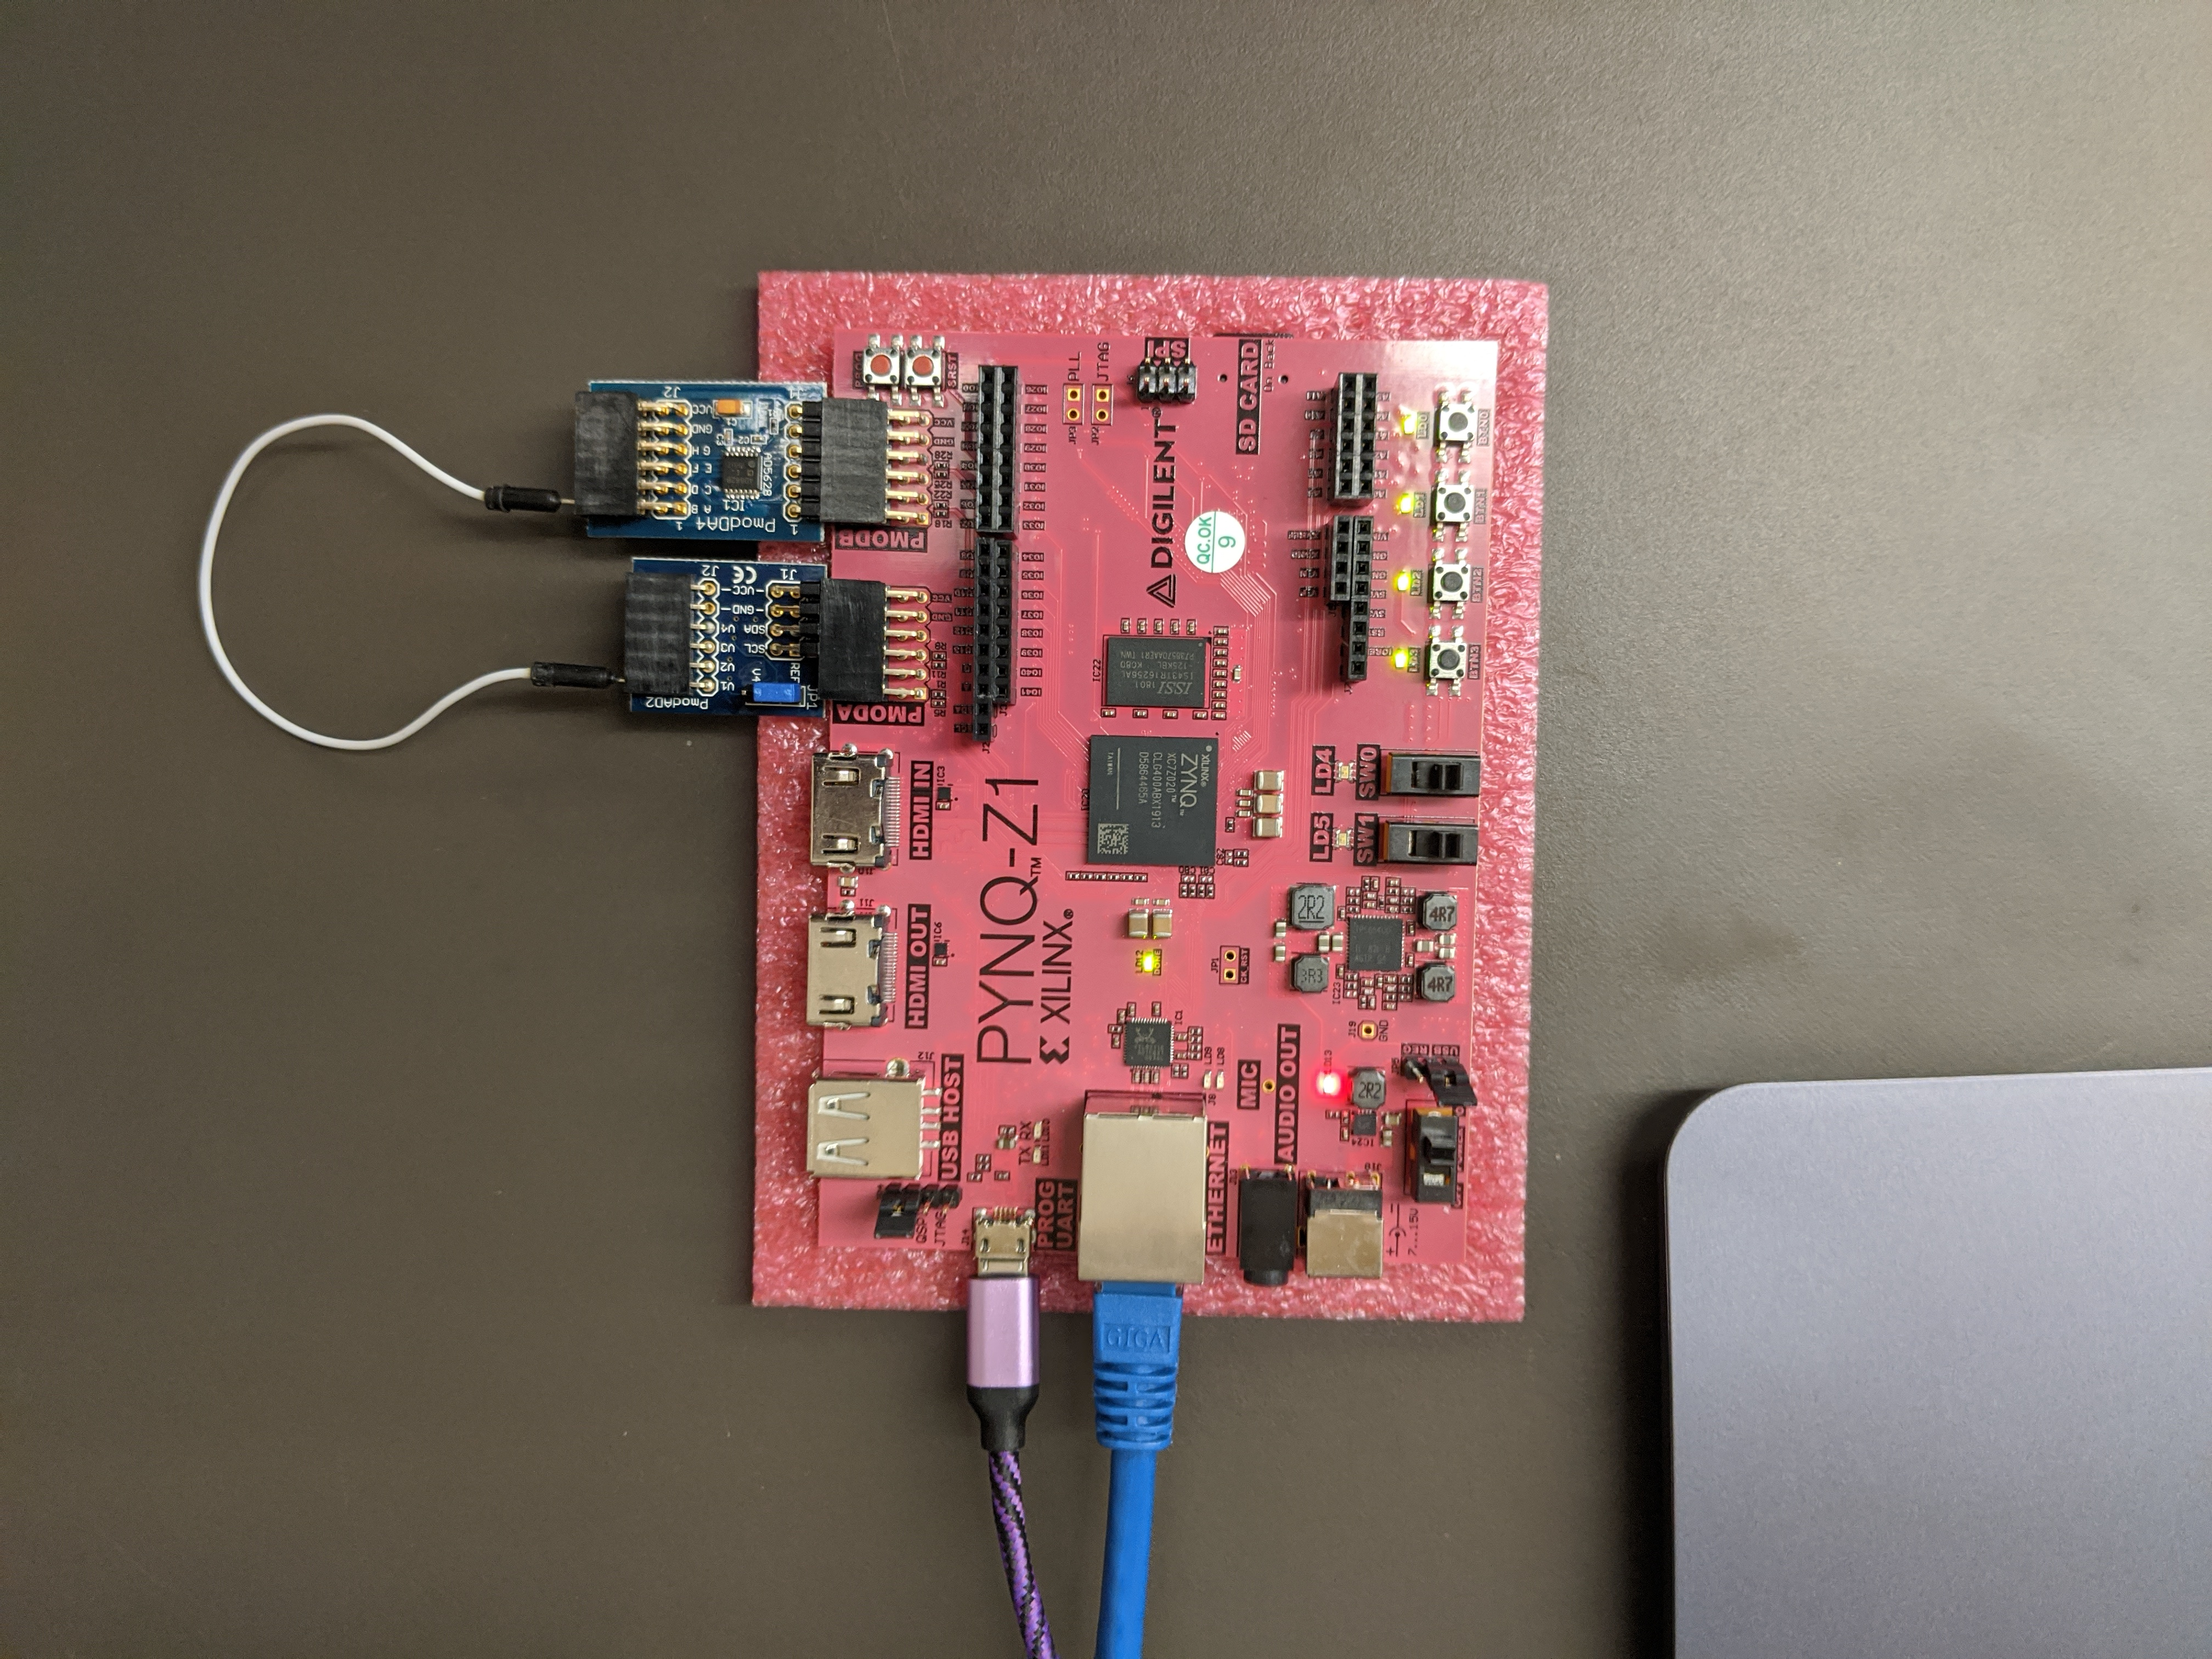
\includegraphics[width=0.65\textwidth]{IMG_20200408_121757.jpg}
\caption{\label{fig:setup1} The PYNQ-Z1 board, along with the AD2 and DA4 Pmods.  The blue objects are the Pmods: the lower one is the ADC and the upper is the DAC.  The ADC has 12-bits of resolution and a range of 0-2V.}
\end{figure}

Consider Fig. \ref{fig:setup1}.  The PYNQ-Z1 is shown as usual, connected to the laptop via USB for power and Ethernet for communications.  The two Pmods are the DAC and the ADC connected with a wire.  The wire carries the analog voltage of the DAC to the ADC.  In the ADC the voltage is digitized and passed from the PL layer to the PS layer.

Navitate to the \verb+getting_started+ folder.  Run the Jupyter script entitled \verb+base_overlay_iop.ipynb+.  The instructions will show you how to send a voltage from the DAC to the ADC via the PMODA and PMODB objects.  Running each of the code cells will show you how to take one voltage, and then scan over the range of the ADC and graph the \textit{expected} output versus the \textit{measured} output.

\section{Modify the Code}

Your task is to figure out how to modify the code in the sections entited \textbf{Tracking the IO Error} and \textbf{Error plot with Matplotlib} to produce a sine wave. Copy and paste the relevant code into a new cell at the bottom, but modify it so that the following criteria are satisfied.

\begin{itemize}
\item A: Do not use the same variable names, so that your results are independent of the code above your additions.
\item B: Notice the role of the \verb+delay+ variable in the original code.  It controls how \textit{often} ADC samples are read from the DAC that just sent them.
\item C: If you make the \verb+delay+ parameter longer, how does this affect the plot of the sine wave?  What is the \textit{frequency of the sine wave?}
\end{itemize}

\section{Implications for Final Projects}

Below are some ideas related to final project design that involve these ADC and DAC Pmods:

\begin{itemize}
\item Sending a voltage over a long cable and testing whether the impedence of the cable affects the ADC reading.
\item Creating code that can use two pynq boards to send and receive analog signals between them.
\item A morse code system between two pynq boards, or with the loopback setup in this lab.
\end{itemize}

\end{document}
